\documentclass{paper}

%\usepackage{times}
\usepackage{epsfig}
\usepackage{graphicx}
\usepackage{amsmath}
\usepackage{amssymb}
\usepackage{color}
\usepackage{caption}
\usepackage{subcaption}
\usepackage{here}

% load package with ``framed'' and ``numbered'' option.
%\usepackage[framed,numbered,autolinebreaks,useliterate]{mcode}

% something NOT relevant to the usage of the package.
\setlength{\parindent}{0pt}
\setlength{\parskip}{18pt}


\usepackage[latin1]{inputenc} 
\usepackage[T1]{fontenc} 

\usepackage{listings} 
\lstset{% 
   language=Matlab, 
   basicstyle=\small\ttfamily, 
} 
\graphicspath{{inpainting/Figures/}}


\title{Assignment 1}
\author{Mich\`{e}le Wyss\\10-104-123}
% //////////////////////////////////////////////////


\begin{document}
\maketitle


% Add figures:
%\begin{figure}[t]
%%\begin{center}
%\quad\quad   \includegraphics[width=1\linewidth]{ass2}
%%\end{center}
%
%\label{fig:performance}
%\end{figure}

\section*{Inpainting}
\subsection*{Problem}
Inpainting is an image processing method that aims for reconstruction of lost or corrupted parts of an image. The goal is to get a plausible-looking image without undefined or invalid pieces.

\subsection*{Motivations}
Sometimes it's a bad thing that some objects appear in a photograph, e.g. as a tourist I'd like to make a picture of a place but some people are standing around and occlude parts of the actual target image. A simple idea is to just remove the persons after the photograph has been taken. This is a typical example of where an image with holes and invalid regions appears. Image inpainting is one possible approach to generate sensible content for those regions that were occluded before.

\subsection*{Derivation of gradient}
Gradient descent is a rather simple iterative approach to minimize a function. Starting at an (randomly chosen)  initial point, the following update rule is performed:

\begin{equation}
\theta_j := \theta_j - \alpha \cdot \frac{\partial}{\partial \theta_j} J(\theta),
\label{eq:update-rule}
\end{equation}
where $\theta_j$ are the unknown parameters of the model, $alpha$ is the \emph{learning rate} and $J(\theta)$ is the gradient of a cost function that is aimed to be minimized.

\noindent For our inpainting problem, we formulate the following cost function:


$$J(u) = \frac{\lambda}{2} \|u-g\|_\Omega^2 + \|\nabla u \|_2.$$
Here, the value $u$ that we optimize for is an image with sensible content, $g$ is the input image containing undefined pieces and $\lambda$ is a regularization parameter to control the tradeoff between exactness of fitting and smoothness of the result. The above update rule will then look as follows:

$$ u[i,j] := u[i,j] - \alpha \cdot \frac{\partial}{\partial u[i,j]} J(u).$$

Clearly, we need to know the derivative $\frac{\partial}{\partial u} J(u)$ to apply gradient descent. It is given by

\begin{align*}
 \frac{\partial}{\partial u[i,j]} \left( \frac{\lambda}{2} \|u-g\|_\Omega^2 + \|\nabla u\|_2 \right) &= \frac{\partial}{\partial u[i,j]} \left( \frac{\lambda}{2} \left(\sum_{i,j} \Omega[i,j] \cdot (u[i,j] - g[i,j])^2\right) + \|\nabla u\|_2 \right) \\
 %
&= \frac{\lambda}{2} \cdot \frac{\partial}{\partial u[i,j]} \left(\sum_{i,j} \Omega[i,j] \cdot (u[i,j] - g[i,j])^2\right) + \frac{\partial}{\partial u[i,j]} \|\nabla u \|_2 \\
%
&= \frac{\lambda}{2} \cdot \frac{\partial}{\partial u[i,j]} \Omega[i,j] \cdot (u[i,j] - g[i,j])^2 + \frac{\partial}{\partial u[i,j]} \|\nabla u \|_2 \\
%
&= \lambda \cdot \Omega[i,j] \cdot (u[i,j] - g[i,j]) + \frac{\partial}{\partial u[i,j]} \|\nabla u \|_2 
\end{align*}

The target image $u$ is 2-dimensional and therefore $\|\nabla u \|_2$ is given by

\begin{equation} \|\nabla u \|_2 = \sum_{i,j} \underbrace{\sqrt{(u[i+1,j] - u [i,j])^2 + (u[i,j+1] - u[i,j])^2}}_{\tau[i,j]}.
 \label{eq:grad}
\end{equation}

Because for fixed $i$ and $j$ most of the summation terms in Equation (\ref{eq:grad}) are constant, the derivative $\frac{\partial}{\partial u[i,j]} \|\nabla u \|_2$ reduces to

$$\frac{\partial}{\partial u[i,j]} \|\nabla u \|_2 = \frac{\partial \tau[i,j]}{\partial u[i,j]} + \frac{\partial \tau[i-1,j]}{\partial u[i,j]} + \frac{\partial \tau[i,j-1]}{\partial u[i,j]}.$$

There are now derivative terms that are left to compute. This can be done straight forward:
\begin{align*}
\frac{\partial \tau[i,j]}{\partial u[i,j]} &= \frac{\partial}{\partial u[i,j]} \sqrt{(u[i+1,j] - u[i,j])^2 + (u[i,j+1] - u[i,j])^2} \\
&= \frac{1}{2} \cdot \frac{1}{\tau[i,j]} \cdot \left((-2) \cdot (u[i+1,j] - u[i,j]) -2 (u[i,j+1] - u[i,j])\right) \\
&= \frac{- ((u[i+1,j] - u[i,j]) + (u[i,j+1] - u[i,j]))}{\tau[i,j]} \\
&= \frac{2 u[i,j] - u[i+1,j] - u[i,j+1]}{\tau[i,j]}, \\
\frac{\partial \tau[i-1,j]}{\partial u[i,j]} &= \frac{\partial}{\partial u[i,j]} \sqrt{(u[i,j] - u[i-1,j])^2 + (u[i-1,j+1] - u[i-1,j])^2} \\
&= \frac{1}{2} \cdot \frac{1}{\tau[i-1,j]} \cdot \left( 2 \cdot (u[i,j] - u[i-1,j]) \right) \\
&= \frac{u[i,j]-u[i-1,j]}{\tau[i-1,j]}, \\
\frac{\partial \tau[i,j-1]}{\partial u[i,j]} &= \frac{\partial}{\partial u[i,j]} \sqrt{(u[i+1,j-1] - u[i,j-1])^2 + (u[i,j] - u[i,j-1])^2} \\
&= \frac{1}{2} \cdot \frac{1}{\tau[i,j-1]} \cdot 2 (u[i,j] - u[i,j-1]) \\
&= \frac{u[i,j] - u[i,j-1]}{\tau[i,j-1]}.
\end{align*}

All in all we have therefore the following update rule:
\begin{equation}
\begin{aligned}
  u[i,j] := u[i,j] - \alpha \cdot \Bigg( \lambda \Omega[i,j] \cdot (u[i,j]-g[i,j]) &+ \frac{2 u[i,j] - u[i+1,j] - u[i,j+1]}{\tau[i,j]} \\ 
  &+ \frac{u[i,j]-u[i-1,j]}{\tau[i-1,j]} \\ 
  &+ \frac{u[i,j] - u[i,j-1]}{\tau[i,j-1]}\Bigg)
\end{aligned}
\label{eq:update-final}
\end{equation}


\subsection*{Implement gradient descent for inpainting}
I implemented inpainting using the mentioned gradient descent method. The gradients were computed as derived above. 
A quite small learning rate of $\alpha$ = 0.0005 ensures that the iterative approach converges -- however, this also leads to the need of many iterations to get an acceptable result.
\begin{figure}[ht]
\centering
\begin{subfigure}[h]{0.45\textwidth}
	\centering
	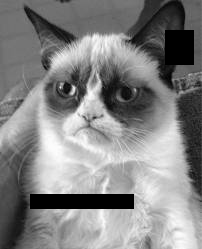
\includegraphics[width=\textwidth]{cat-input}
	\caption*{Input}
\end{subfigure}
~
\begin{subfigure}[h]{0.45\textwidth}
	\centering
	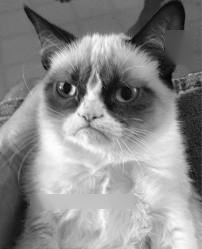
\includegraphics[width=\textwidth]{cat-iter100000-lambda1000-alpha0_0005}
	\caption*{Output ($100'000$ iterations)}
\end{subfigure}

\vspace{3mm}
\begin{subfigure}[h]{0.3\textwidth}
	\centering
	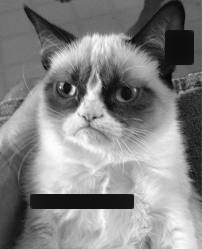
\includegraphics[width=\textwidth]{cat-iter1000-lambda1000-alpha0_0005}
	\caption*{$1000$ iterations}
\end{subfigure}
~
\begin{subfigure}[h]{0.3\textwidth}
	\centering
	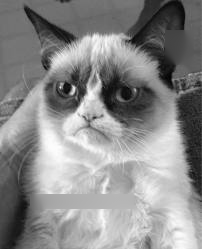
\includegraphics[width=\textwidth]{cat-iter10000-lambda1000-alpha0_0005}
	\caption*{$10'000$ iterations}
\end{subfigure}
~
\begin{subfigure}[h]{0.3\textwidth}
	\centering
	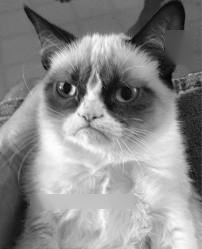
\includegraphics[width=\textwidth]{cat-iter50000-lambda1000-alpha0_0005}
	\caption*{$50'000$ iterations}
\end{subfigure}
\label{fig:results-cat}
\end{figure}
 
Another example:
\begin{figure}[ht]
\centering
\begin{subfigure}[h]{0.45\textwidth}
	\centering
	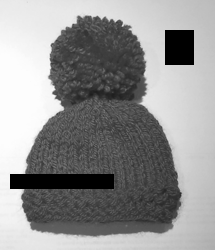
\includegraphics[width=\textwidth]{hat-input}
	\caption*{Input}
\end{subfigure}
~
\begin{subfigure}[h]{0.45\textwidth}
	\centering
	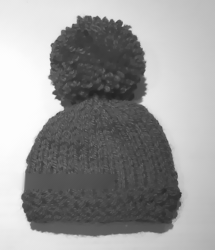
\includegraphics[width=\textwidth]{hat-iter50000-lambda100-alpha0_001}
	\caption*{Output ($50'000$ iterations)}
\end{subfigure}

\vspace{3mm}
\begin{subfigure}[h]{0.3\textwidth}
	\centering
	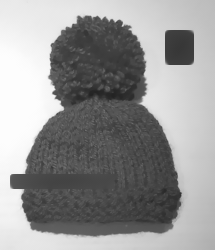
\includegraphics[width=\textwidth]{hat-iter2000-lambda100-alpha0_001}
	\caption*{$2'000$ iterations}
\end{subfigure}
~
\begin{subfigure}[h]{0.3\textwidth}
	\centering
	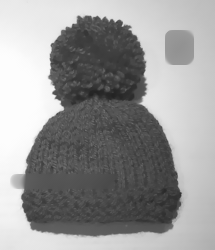
\includegraphics[width=\textwidth]{hat-iter5000-lambda100-alpha0_001}
	\caption*{$5'000$ iterations}
\end{subfigure}
~
\begin{subfigure}[h]{0.3\textwidth}
	\centering
	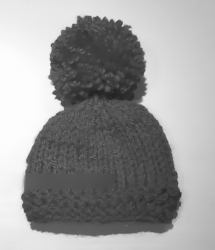
\includegraphics[width=\textwidth]{hat-iter10000-lambda100-alpha0_001}
	\caption*{$10'000$ iterations}
\end{subfigure}
\label{fig:results-hat}
\end{figure}

\subsection*{The effect of $\lambda$}
In the objective function
$$J(u) = \frac{\lambda}{2} \|u-g\|_\Omega^2 + \|\nabla u \|_2$$
the parameter $\lambda$ is a \emph{regularization parameter}. It controls the tradeoff between the two constraints of fitting the image and keeping the result smooth. A very low $\lambda$, e.g. $\lambda = 0.1$ leads to an oversmoothed image whereas a very large value for $\lambda$ may possibly fail to reach a nice-looking (smooth) image (see Figure \ref{fig:lambda-values}). Moreover, a large lambda-value generally requires a smaller learning rate $\alpha$. This can be seen directly by considering the final update rule (\ref{eq:update-final}) from the fact that the first term gets a high weight and may cause the gradient descent method to diverge.

\begin{figure}[h]
\centering
\begin{subfigure}[h]{0.3\textwidth}
	\centering
	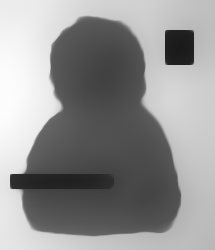
\includegraphics[width=\textwidth]{hat-iter1000-lambda0_1-alpha0_001}
	\caption*{1'000 iterations, $\lambda = 0.1$}
\end{subfigure}
~
\begin{subfigure}[h]{0.3\textwidth}
	\centering
	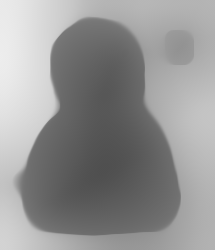
\includegraphics[width=\textwidth]{hat-iter5000-lambda0_1-alpha0_001}
	\caption*{5'000 iterations, $\lambda = 0.1$}
\end{subfigure}
~
\begin{subfigure}[h]{0.3\textwidth}
	\centering
	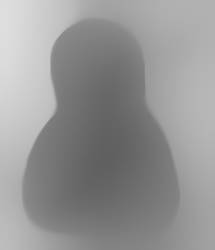
\includegraphics[width=\textwidth]{hat-iter10000-lambda0_1-alpha0_001}
	\caption*{$10'000$ iterations, $\lambda = 0.1$}
\end{subfigure}

\vspace{3mm}
\begin{subfigure}[h]{0.3\textwidth}
	\centering
	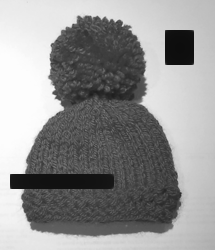
\includegraphics[width=\textwidth]{hat-iter5000-lambda10000-alpha0_0001}
	\caption*{$5'000$ iterations}
\end{subfigure}
~
\begin{subfigure}[h]{0.3\textwidth}
	\centering
	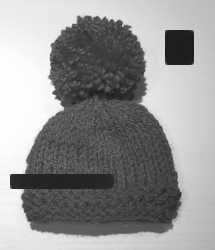
\includegraphics[width=\textwidth]{hat-iter10000-lambda10000-alpha0_0001}
	\caption*{$10'000$ iterations}
\end{subfigure}
~
\begin{subfigure}[h]{0.3\textwidth}
	\centering
	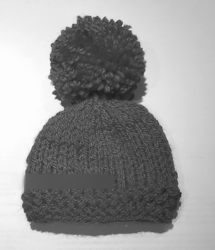
\includegraphics[width=\textwidth]{hat-iter100000-lambda10000-alpha0_0001}
	\caption*{$100'000$ iterations}
\end{subfigure}
\caption{Top row: results obtained with $\lambda = 0.1$. Bottom row: results obtained with $\lambda = 10'000$.}
\label{fig:lambda-values}
\end{figure}

\begin{enumerate}
\item \textbf{Derivation of gradient.} In this section you should:

\begin{itemize}
\item Write the finite difference approximation of the objective function $E$.
\item Compute the gradient of the objective function $\nabla_uE$.  
\end{itemize}


\item \textbf{Implement gradient descent for inpainting.} In this section you should:

\begin{itemize}
\item Show some images, as the the gradient method progresses iteration by iteration. Display the initial and the final image and 3 more images in between.
\end{itemize}

\item \textbf{Show images obtained by very high, very low and optimal $\lambda$.} In this section you should:

\begin{itemize}
\item Display 3 images with different $\lambda$ (very low, very high and optimal).
\item Describe the effect of $\lambda$ on the solution.
\end{itemize}

\item \textbf{ Find optimal $\lambda$.} In this section you should:

\begin{itemize}
\item Display the $SSD$ vs. $\lambda$ graph.
\item Describe the effect of $\lambda$ with respect to the $SSD$ between the ground truth and the solution image.
\end{itemize}
\end{enumerate}


 \end{document}
 
 